\section{Changing the System Bounds}
\subsection{Disturbance Rejection and Input Saturation}

This section will look at the proposed changes stated in Section~\ref{sec:Analysis for acceptable control:disturbances}. Since there is no information on the current controllers and final control elements employed on site, investigation into changes of the control hardware will not be conducted. This is purely due to

\begin{enumerate}
	\item Lack of information about current control infrastructure. 
	\item Lack of a first principles mathematical model, or Aspen simulation where the sizes of the control elements can be changed at will without any additional cost.
\end{enumerate}

The proposed changes to the perimeters of the control system will therefore be investigated. As mentioned in Section~\ref{sec:Analysis for acceptable control:disturbances}, disturbance rejection is required for a too high range of both disturbances. In order to rectify the situation, the ranges where adjusted. This in turn caused the scaled system to change, and new responses resulted. Table~\ref{tab:Disturbance_variables_updated_scaling} contains more information with regard to the proposed ranges.

\begin{table}[H]
	\centering
	\caption{The new proposed boundaries of the disturbance variables in the system.}
	\begin{tabular}{cccc}
		\hline
		\textbf{\begin{tabular}[c]{@{}c@{}}Disturbance\\   Variable\end{tabular}} & \textbf{\begin{tabular}[c]{@{}c@{}}Lower \\ Constraint\end{tabular}} & \textbf{\begin{tabular}[c]{@{}c@{}}Upper \\ Constraint\end{tabular}} & \textbf{\begin{tabular}[c]{@{}c@{}}Steady State \\ Value\end{tabular}} \\\hline
		d1, Feed Flow Rate            & 0.65                       & 1.0                       & 0.8                         \\
		d2, Feed Temperature          & 60                        & 95                       & 78                         
		\\\hline      
	\end{tabular}
	\label{tab:Disturbance_variables_updated_scaling}
\end{table}

This led to a new scaling matrix

\begin{equation}
	D_d = \begin{bmatrix}
	0.2 & 0 \\
	0 & 18\\
	\end{bmatrix}
\end{equation}

and a new disturbance matrix

\begin{equation}
G_d(s) = \begin{bmatrix}
G_{d11} & G_{d12} \\
G_{d21} & G_{d22} \\
G_{d31} & G_{d32} \\
\end{bmatrix} = \begin{bmatrix}
\frac{2.8e^{-12s}}{6.2s+1} & \frac{-1800(0.028952s+0.0011)e^{-2.66s}}{(7.85s+1)(4.63s+1)} \\
\frac{10.6e^{-10.5s}}{6.9s+1} & \frac{-1800(-0.062784s+0.0032)e^{-3.44s}}{(7.29s+1)(8.94s+1)} \\
\frac{-0.577e^{-0.6s}}{7.01s+1} & \frac{1.44e^{-2.6s}}{7.76s+1}
\end{bmatrix}
\end{equation}

The same mathematical procedure is then followed as outlined in Section~\ref{sec:Analysis for acceptable control:disturbances}, to establish whether acceptable disturbance rejection can take place. The following figures result.

\begin{figure}[H]
	\centering
	\includegraphics[width=0.7\linewidth]{"Figures/Disturbance Analysis 2 Max Norm_Updated"}
	\caption{The effect of disturbances on input saturation.}
	\label{fig:disturbance-analysis-2-max-norm_updated}
\end{figure}

 \begin{figure}[H]
	\centering
	\begin{minipage}{.48\textwidth}
		\centering
		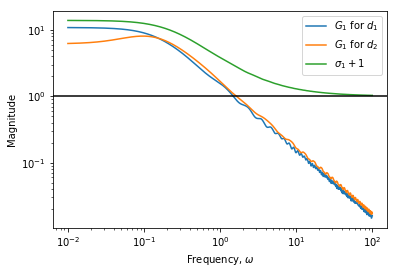
\includegraphics[width=\linewidth]{Figures/InputSaturation1_Updated}
		\captionof{figure}{Graphical representation of criteria outlined in Equation~\ref{eq:Input saturation of disturbances}, for $e_1$}
		\label{fig:Input Saturation 1_Updated}
	\end{minipage}%
	\hfill
	\begin{minipage}{.48\textwidth}
		\centering
		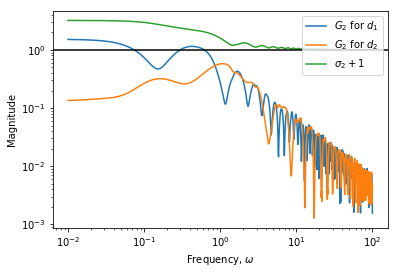
\includegraphics[width=\linewidth]{Figures/InputSaturation2_Updated}
		\captionof{figure}{Graphical representation of criteria outlined in Equation~\ref{eq:Input saturation of disturbances}, for $e_2$}
		\label{fig:Input Saturation 2_Updated}
	\end{minipage}
\end{figure}

\begin{figure}[H]
	\centering
	\begin{minipage}{.48\textwidth}
		\centering
		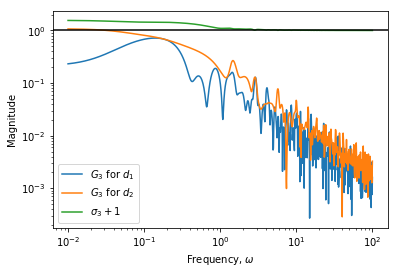
\includegraphics[width=\linewidth]{Figures/InputSaturation3_Updated}
		\captionof{figure}{Graphical representation of criteria outlined in Equation~\ref{eq:Input saturation of disturbances}, for $e_3$}
		\label{fig:Input Saturation 3_Updated}
	\end{minipage}%
	\hfill
	\begin{minipage}{.48\textwidth}
		\centering
		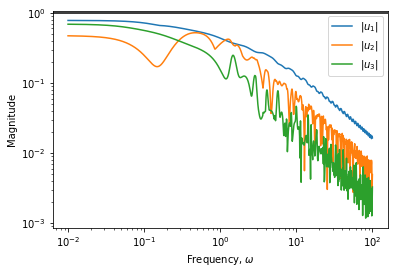
\includegraphics[width=\linewidth]{Figures/Input_Requirements_Updated}
		\captionof{figure}{The required controller input values for the worst case }
		\label{fig:Input Requirements_Updated}
	\end{minipage}
\end{figure}